\documentclass[10pt,a4paper]{article}

% ============================================================================
%  TP1 Optimización 2026 2C — "Portafolio de Productos Pastarazzi"
%  Martínez Folica, Nazareno · Naón, Pedro
% ============================================================================

\usepackage[utf8]{inputenc}
\usepackage[T1]{fontenc}
\usepackage{lmodern}
\usepackage[a4paper,margin=2.2cm,headheight=14pt]{geometry}
\usepackage{graphicx}
\usepackage{booktabs}
\usepackage{array}
\usepackage{tabularx}
\usepackage{longtable}
\usepackage[table]{xcolor}
\usepackage{amsmath}
\usepackage{amssymb}
\usepackage{enumitem}
\usepackage{caption}
\captionsetup{font=small,skip=4pt}
\usepackage{fancyhdr}
\usepackage{titlesec}
\usepackage{tikz}
\usetikzlibrary{arrows.meta,calc,positioning}
\usepackage[colorlinks=true,linkcolor=accentlink,citecolor=accentlink,urlcolor=accentlink,linktoc=all]{hyperref}

% ---------- paleta ----------------------------------------------------------
\definecolor{doncarlo}{HTML}{C0504D}
\definecolor{agnellis}{HTML}{4F81BD}
\definecolor{triguetti}{HTML}{9BBB59}
\definecolor{candealix}{HTML}{8064A2}
\definecolor{rena}{HTML}{F79646}
\definecolor{accent}{HTML}{1F4E79}
\definecolor{accentlink}{HTML}{1F5C99}
\definecolor{filagris}{HTML}{F2F2F2}

% ---------- tipografía de títulos -------------------------------------------
\titleformat{\section}{\normalfont\Large\bfseries\color{accent}}{\thesection}{0.6em}{}
\titleformat{\subsection}{\normalfont\large\bfseries\color{accent}}{\thesubsection}{0.6em}{}
\titleformat{\subsubsection}{\normalfont\bfseries\color{accent}}{\thesubsubsection}{0.6em}{}
\titlespacing*{\section}{0pt}{1.1em}{0.55em}
\titlespacing*{\subsection}{0pt}{0.9em}{0.4em}

% ---------- flotantes ------------------------------------------------------
% El documento tiene 14 tablas y 6 figuras. Los valores por defecto de LaTeX
% son conservadores (topfraction .7 / textfraction .2) y con esta densidad
% empujan las tablas varias paginas lejos del texto que las comenta. Estos
% valores permiten mas area de flotante por pagina sin llegar a paginas
% compuestas solo de tablas.
\renewcommand{\topfraction}{0.9}
\renewcommand{\bottomfraction}{0.7}
\renewcommand{\textfraction}{0.1}
\renewcommand{\floatpagefraction}{0.75}
\setcounter{topnumber}{3}
\setcounter{totalnumber}{5}

\pagestyle{fancy}
\fancyhf{}
\renewcommand{\headrulewidth}{0.4pt}
\fancyhead[L]{\small Optimización 2026 2C — TP1 Pastarazzi}
\fancyhead[R]{\small Martínez Folica, N. · Naón, P.}
\fancyfoot[C]{\small\thepage}

\setlength{\parskip}{0.25em}
\setlist[itemize]{topsep=0.2em, itemsep=0.05em}
\setlist[enumerate]{topsep=0.2em, itemsep=0.05em}

\newcommand{\marca}[2]{\textcolor{#1}{\rule{0.28cm}{0.28cm}}~#2}
\newcommand{\MM}{\,\text{\$MM}}

\renewcommand{\contentsname}{Índice}
\renewcommand{\figurename}{Figura}
\renewcommand{\tablename}{Tabla}

\begin{document}

% ============================================================================
\begin{titlepage}
\begin{center}
\vspace*{1.2cm}
{\large UCA}\\[2pt]
{\large Facultad de Ingeniería y Ciencias Agrarias}\\[1.4cm]

{\large Optimización — 2026, 2\textdegree{} Cuatrimestre}\\[0.3cm]
{\large Trabajo Práctico N.\textdegree{} 1}\\[1.8cm]

\rule{0.85\linewidth}{0.6pt}\\[0.5cm]
{\Huge\bfseries\color{accent} Portafolio de Productos Pastarazzi}\\[0.5cm]
{\Large Modelado de programación lineal y análisis de sensibilidad\\ de un plan de inversión en marketing}\\[0.5cm]
\rule{0.85\linewidth}{0.6pt}\\[2.2cm]

\begin{tabular}{c}
{\large\bfseries Integrantes} \\[0.4cm]
{\large Martínez Folica, Nazareno} \\[0.15cm]
{\large Naón, Pedro}
\end{tabular}

\vfill

{\large 7 de septiembre de 2026}
\end{center}
\end{titlepage}

\pagenumbering{roman}
\tableofcontents
\newpage
\pagenumbering{arabic}

% ============================================================================
\section*{Introducción}
\addcontentsline{toc}{section}{Introducción}

Pastarazzi es una fabricante de pastas secas con cinco marcas —Don Carlo, Agnellis,
Triguetti, Candealix y Rena Speziale— que compiten en distintos segmentos del
mercado. Para la próxima campaña, la empresa cuenta con \$17.000 millones de
presupuesto de marketing y tiene que decidir cómo repartirlo, según plantea el
enunciado del trabajo práctico \cite{consigna}. No hay plata para lanzar
productos nuevos, así que la única palanca disponible es la combinación entre
las cinco líneas ya existentes.

Detrás de esa decisión hay una tensión real dentro del directorio: los
accionistas, golpeados por trimestres flojos, piden rentabilidad inmediata;
el equipo directivo, en cambio, empuja una ofensiva comercial sostenida, entre
otras cosas porque sus bonos dependen de los ingresos totales de la compañía y no
de la ganancia. A esa tensión se le suman una serie de reglas de negocio ya
fijadas —paridad entre Don Carlo y Agnellis, un piso mínimo para Triguetti, un
mínimo relativo para Rena Speziale— que hay que respetar sí o sí.

Este informe construye un modelo de programación lineal para ese problema, lo
resuelve, y usa el análisis de sensibilidad para entender no solo \emph{cuál}
es el plan óptimo sino \emph{por qué} es óptimo y qué tan firme es frente a los
datos que el enunciado no terminaba de precisar. El documento sigue la
estructura que pide la cátedra \cite{catedra-clases} (modelo, sensibilidad,
esquema del proceso y herramientas) y cierra respondiendo, con esos mismos
números, las cuatro consultas concretas que el directorio le hizo al equipo de
análisis.

Una aclaración que conviene hacer de entrada: la consigna del TP tiene dos
listas distintas, ambas numeradas con las letras a) a d). La primera, en la
página 1, describe \emph{cómo} tiene que estar armado este informe (el modelo,
la sensibilidad, el esquema, las librerías). La segunda, en la página 4,
son las \emph{cuatro consultas} que el directorio le hace al equipo de
análisis. Para no confundirlas, en este documento la primera lista organiza las
Secciones 1 a 4, y la segunda se responde en la Sección 5, bajo el nombre de
``consultas'' y no de letras.

% ============================================================================
\section{Modelo de programación lineal}

\subsection{Supuestos más importantes}
\label{sec:supuestos}

El enunciado da información abundante pero deliberadamente incompleta en
varios puntos —es, de hecho, uno de los criterios de evaluación explícitos:
``explorar'' significa completar esos huecos con criterio propio. Cada
supuesto que se adoptó responde a tres preguntas: para qué hace falta, por qué
se eligió ese valor y no otro, y cómo se comprobó si importaba. La comprobación
completa está en la Sección~\ref{sec:sensibilidad}; acá se presentan los
supuestos y su justificación.

\begin{itemize}
  \item[\textbf{S1}] \textbf{Tasa de captación de Triguetti en su primer tramo:
    200 clientes por \$MM.} El enunciado da el punto de saturación de Triguetti
    (\$6.000\,MM) pero nunca la tasa a la que capta clientes antes de saturar,
    y sin ese número no se puede calcular nada de la marca. Triguetti compite
    en el mismo segmento que Candealix, que capta 300 clientes por \$MM en su
    primer tramo; como el enunciado le atribuye a Triguetti ``menor elasticidad
    a la inversión'', su tasa tiene que ser menor a 300, pero no puede ser 0
    porque entonces no tendría sentido hablar de un punto de saturación. Se
    adoptó 200 como valor intermedio conservador (dos tercios de la eficiencia
    de Candealix), testeado en el rango 140--260.

  \item[\textbf{S2}] \textbf{Tasa de captura de billetera: 100\,\%.} Se asume
    que un cliente nuevo destina todo su gasto anual en pastas a la marca que
    lo captó. Es una simplificación que probablemente sobreestima el retorno
    del marketing —en la práctica, un consumidor reparte entre marcas—, así
    que se testea contra el 70\,\%.

  \item[\textbf{S3}] \textbf{Los márgenes de la Fig.~1 del enunciado son
    exactos.} El propio enunciado los llama ``un estimado'', así que se
    barrieron $\pm30\,\%$ uno por uno para ver si el ranking de rentabilidad
    entre marcas se sostiene.

  \item[\textbf{S4}] \textbf{Las tasas de captación y los umbrales de tramo son
    exactos.} El enunciado usa lenguaje deliberadamente vago en todas
    (``alrededor de 500'', ``cerca de 400'', ``aproximadamente \$6.000
    millones''...). Se barrieron $\pm30\,\%$ para identificar cuál mueve más
    el resultado.

  \item[\textbf{S5}] \textbf{Cada marca capta clientes nuevos en un único
    segmento: el de su posicionamiento de producto.} La Fig.~2 muestra que cada
    marca \emph{vende} en varios segmentos, pero la tasa de captación es un
    solo número por marca, y sin decidir a qué segmento va un cliente nuevo no
    se sabe si gasta \$41.000 o \$134.000 al año. Se adoptó que Don Carlo y
    Agnellis captan en el segmento bajo, Triguetti y Candealix en el medio, y
    Rena Speziale en el alto —coherente con el propio texto (``el segmento de
    gama baja está dominado por Don Carlo'', ``Rena Speziale... en la gama
    alta'') y con que el enunciado mide el tope del 65\,\% justamente contra
    ``el mercado de menor poder adquisitivo''. Es, de los nueve supuestos, el
    que más resultados toca (Tabla~\ref{tab:mapa_supuestos}), y se lo testea
    contra una lectura alternativa en la Sección~\ref{sec:b2}.

  \item[\textbf{S6}] \textbf{La regla de paridad Don Carlo/Agnellis se lee como
    igualdad de inversión: $x_{DC}=x_{AG}$.} La frase del enunciado (``el otro
    debe recibir un refuerzo de igual magnitud de inversión'') admite en
    principio una lectura sobre \emph{incrementos} respecto de una campaña
    anterior, pero esa campaña anterior no está en los datos, así que la única
    lectura calculable es la de inversión total. Es, además, exactamente el
    supuesto que la Consulta~2 del directorio pide relajar.

  \item[\textbf{S7}] \textbf{Las reglas de Triguetti y Rena se leen como
    piso, no como cuota exacta.} El 30\,\% de Triguetti se calcula sobre el
    presupuesto total (\$17.000\,MM) y se exige como mínimo (``$\geq$''); la
    regla del doble de Rena también se lee como mínimo. Ambas lecturas se
    contrastan contra sus alternativas en la Sección~\ref{sec:sensibilidad}.

  \item[\textbf{S8}] \textbf{El presupuesto de marketing es un recurso a
    asignar, no un costo que se resta de la utilidad.} Si el margen operativo
    ya contempla el gasto comercial, restar además la inversión sería contar
    el mismo gasto dos veces. Como el monto total (\$17.000\,MM) es igual en
    todos los planes que se comparan, esta decisión no cambia el óptimo; sí
    cambia el número que se reporta como ``utilidad'', y eso se aclara cada vez
    que corresponde.

  \item[\textbf{S9}] \textbf{Supuestos de menor impacto, declarados y no
    testeados individualmente:} la facturación de base (la que la empresa
    factura sin invertir un peso) se conserva y la campaña se suma por
    encima de ella; a falta de una definición de ``canal de venta'' en los
    datos, se usa el segmento de mercado (bajo/medio/alto) como proxy; el
    horizonte es de un año sin estacionalidad; y rigen los cinco supuestos
    generales de todo modelo de PL (proporcionalidad, aditividad,
    divisibilidad, certidumbre y no negatividad), con dos salvedades que se
    tratan explícitamente más abajo: la divisibilidad se relaja en el umbral
    de Candealix (\S\ref{sec:restricciones}) y la proporcionalidad se rompe a
    propósito en los rendimientos decrecientes, resuelta con tramos lineales
    (\S\ref{sec:variables}).
\end{itemize}

\begin{table}[htbp]
\centering
\small
\caption{Qué tan crítico es cada supuesto para cada consulta del directorio.}
\label{tab:mapa_supuestos}
\begin{tabular}{lcccc}
\toprule
\textbf{Supuesto} & \textbf{Consulta 1} & \textbf{Consulta 2} & \textbf{Consulta 3} & \textbf{Consulta 4} \\
\midrule
S1 — tasa Triguetti          & \textbullet     & $\circ$         & \textbullet     & \textbullet\textbullet \\
S2 — captura de billetera    & \textbullet\textbullet & \textbullet & \textbullet   & $\circ$ \\
S3 — márgenes                & \textbullet     & \textbullet     & \textbullet\textbullet & \textbullet \\
S4 — tasas de captación      & \textbullet     & \textbullet\textbullet & \textbullet & \textbullet \\
S5 — segmento de captación   & \textbullet\textbullet & \textbullet\textbullet & \textbullet\textbullet & \textbullet \\
S6 — lectura de la paridad   & \textbullet     & \textbullet\textbullet & $\circ$       & $\circ$ \\
S7 — lectura de los pisos    & \textbullet     & $\circ$         & \textbullet     & \textbullet\textbullet \\
S8 — presupuesto en el funcional & \textbullet & $\circ$         & \textbullet     & $\circ$ \\
\bottomrule
\end{tabular}
\vspace{2mm}\\
\small\textbullet\textbullet\ crítico \quad \textbullet\ relevante \quad $\circ$\ indiferente
\vspace{1mm}\\
\footnotesize S9 no aparece en la tabla porque no es un supuesto único sino un
conjunto de decisiones menores, declaradas y no testeadas individualmente.
\end{table}

\subsection{Variables de decisión}
\label{sec:variables}

La variable de decisión central es cuánto invertir en marketing en cada marca,
en millones de pesos:
\[
x_{DC},\ x_{AG},\ x_{TRI},\ x_{CAN},\ x_{RS} \ \geq 0
\]
Se trabaja en millones de pesos porque las tasas de captación vienen dadas en
``clientes por millón invertido'': hacerlo en pesos corrientes obligaría a
arrastrar factores de $10^6$ por todo el modelo sin ganar nada a cambio.

Tres de las cinco marcas —Candealix, Rena Speziale y, con la tasa asumida en
S1, también Triguetti— tienen \textbf{rendimientos decrecientes}: los primeros
pesos invertidos captan clientes a una tasa, y superado un umbral, a una tasa
menor. Para modelar eso sin salir de la programación lineal, la inversión de
esas marcas se separa en tramos:
\[
x_{TRI} = x_{TRI,1} + x_{TRI,2}, \qquad
x_{CAN} = x_{CAN,1} + x_{CAN,2} + x_{CAN,3}, \qquad
x_{RS} = x_{RS,1} + x_{RS,2} + x_{RS,3}
\]
donde el último tramo de cada una es un tramo de \emph{desperdicio}: tasa de
captación cero y sin tope. Este tramo no estaba en el plan de trabajo original
y se agregó durante la implementación al toparse con un resultado imposible
(se explica en el Recuadro~\ref{box:r10}); representa la plata que, por las
reglas del propio directorio, hay que invertir aunque ya no quede nadie a quien
captar.

Como la curva de captación de cada marca es \textbf{cóncava} —cada tramo rinde
menos que el anterior—, no hacen falta variables binarias para forzar al
solver a llenar primero el tramo más eficiente: al maximizar, cualquier plan
que use el tramo malo teniendo lugar en el bueno es dominado, así que el orden
correcto sale solo. Si los rendimientos fueran \emph{crecientes} (economías de
escala), la curva sería convexa y ahí sí haría falta un modelo de programación
lineal entera mixta.

Además de las variables de inversión, se reportan —pero no se deciden—
tres cantidades derivadas: los clientes nuevos captados, la facturación total
resultante (base más incremental) y la utilidad de cada marca.

\subsection{Función objetivo}
\label{sec:objetivo}

Acá está el corazón del conflicto entre accionistas y directivos: maximizar
utilidad y maximizar facturación son dos funciones objetivo distintas, que en
general dan planes distintos. El modelo se construyó para poder correr las
tres miradas con el mismo código, cambiando solo qué se maximiza.

En los tres casos el funcional se separa en dos partes: una \textbf{constante},
la utilidad o facturación que la empresa ya tiene sin invertir un peso más
(no afecta al óptimo, pero sin ella los números no tienen sentido de negocio),
y una parte \textbf{variable}, que es lo único que el solver decide.

\paragraph{Utilidad neta (la mirada de los accionistas).}
\[
\begin{aligned}
\text{Max } Z_{neta} = \ & 55.421{,}52
+ 0{,}8200\,x_{DC} + 1{,}5375\,x_{AG} \\
& + 1{,}0440\,x_{TRI,1} + 0\cdot x_{TRI,2} \\
& + 1{,}3920\,x_{CAN,1} + 0{,}9280\,x_{CAN,2} + 0\cdot x_{CAN,3}\\
& + 2{,}0100\,x_{RS,1} + 1{,}3400\,x_{RS,2} + 0\cdot x_{RS,3}
\end{aligned}
\]

\paragraph{Utilidad operativa.} Misma estructura, cambiando el margen neto por
el operativo:
\[
\begin{aligned}
\text{Max } Z_{oper} = \ & 80.740{,}39
+ 1{,}4760\,x_{DC} + 2{,}0500\,x_{AG} \\
& + 1{,}2992\,x_{TRI,1} + 1{,}9314\,x_{CAN,1} + 1{,}2876\,x_{CAN,2} \\
& + 3{,}2160\,x_{RS,1} + 2{,}1440\,x_{RS,2}
\end{aligned}
\]

\paragraph{Facturación (la mirada del directorio, ligada a sus bonos).}
\[
\begin{aligned}
\text{Max } Z_{fact} = \ & 797.107
+ 16{,}40\,x_{DC} + 20{,}50\,x_{AG} \\
& + 11{,}60\,x_{TRI,1} + 17{,}40\,x_{CAN,1} + 11{,}60\,x_{CAN,2} \\
& + 20{,}10\,x_{RS,1} + 13{,}40\,x_{RS,2}
\end{aligned}
\]

Como el mercado total de pastas (\$1.657.100\,MM) es una constante, maximizar
facturación es matemáticamente lo mismo que maximizar market share.

Comparando los dos funcionales de utilidad, el \textbf{ranking de las marcas
cambia según qué margen se use}: con margen neto, Don Carlo (0,82) es la peor inversión
marginal del portafolio; con margen operativo (1,476) le gana a Triguetti y al
segundo tramo de Candealix. La elección del margen no es un detalle contable:
cambia qué conviene priorizar, y por eso se corren y se comparan las dos
versiones.

Un coeficiente, a modo de ejemplo de cómo se arma cada uno (Agnellis, margen
neto):
\[
\begin{aligned}
&\underbrace{500\ \tfrac{\text{clientes}}{\text{\$MM}}}_{\text{tasa (enunciado)}}
\times
\underbrace{\$41.000\ \tfrac{}{\text{cliente-año}}}_{\text{gasto del segmento bajo}}
\div 10^6
= 20{,}50 \tfrac{\$MM\text{ fact.}}{\$MM\text{ inv.}} \\[4pt]
&\Longrightarrow\quad
20{,}50 \times 7{,}5\,\% = 1{,}5375 \tfrac{\$MM\text{ util.}}{\$MM\text{ inv.}}
\end{aligned}
\]

\subsection{Parámetros}
\label{sec:parametros}

Los parámetros de entrada son los que trae el enunciado (precios, márgenes,
market share inicial, tamaño de mercado y tasas de captación); de ellos se
derivan cuatro tablas que alimentan directamente el modelo.

\begin{table}[htbp]
\centering\small
\caption{Tamaño del mercado por segmento, en \$MM/año (TAM $\times$ gasto anual por persona).}
\begin{tabular}{lrr}
\toprule
Segmento & TAM (personas) & Mercado (\$MM/año) \\
\midrule
Bajo  & 21.500.000 & 881.500 \\
Medio & 10.600.000 & 614.800 \\
Alto  &  1.200.000 & 160.800 \\
\midrule
\textbf{Total} & \textbf{33.300.000} & \textbf{1.657.100} \\
\bottomrule
\end{tabular}
\end{table}

\begin{table}[htbp]
\centering\small
\caption{Facturación base de cada marca (antes de invertir un peso en la campaña).}
\begin{tabular}{lrr}
\toprule
Marca & Facturación base (\$MM/año) & \% de la facturación \\
\midrule
\marca{doncarlo}{Don Carlo}      & 320.821 & 40{,}2\,\% \\
\marca{agnellis}{Agnellis}       & 192.626 & 24{,}2\,\% \\
\marca{triguetti}{Triguetti}     & 186.048 & 23{,}3\,\% \\
\marca{candealix}{Candealix}     &  78.600 &  9{,}9\,\% \\
\marca{rena}{Rena Speziale}      &  19.012 &  2{,}4\,\% \\
\midrule
\textbf{Total} & \textbf{797.107} & \textbf{100\,\%} \\
\bottomrule
\end{tabular}
\vspace{1mm}\\
\footnotesize Market share inicial de Pastarazzi: $797.107 / 1.657.100 = 48{,}10\,\%$.
\end{table}

\begin{table}[htbp]
\centering\small
\caption{Utilidad neta que genera cada \$MM invertido, por marca y tramo.}
\label{tab:utilidad_millon}
\begin{tabular}{lrr}
\toprule
Marca (tramo) & Facturación por \$MM & Utilidad neta por \$MM \\
\midrule
\marca{rena}{Rena Speziale} (1\textsuperscript{er} tramo)  & 20{,}10 & \textbf{2{,}010} \\
\marca{agnellis}{Agnellis}                                  & 20{,}50 & \textbf{1{,}538} \\
\marca{candealix}{Candealix} (1\textsuperscript{er} tramo)  & 17{,}40 & \textbf{1{,}392} \\
\marca{rena}{Rena Speziale} (2\textsuperscript{do} tramo)   & 13{,}40 & \textbf{1{,}340} \\
\marca{triguetti}{Triguetti} (1\textsuperscript{er} tramo)  & 11{,}60 & \textbf{1{,}044} \\
\marca{candealix}{Candealix} (2\textsuperscript{do} tramo)  & 11{,}60 & \textbf{0{,}928} \\
\marca{doncarlo}{Don Carlo}                                 & 16{,}40 & \textbf{0{,}820} \\
\marca{triguetti}{Triguetti} (2\textsuperscript{do} tramo)  & 0{,}00  & \textbf{0{,}000} \\
\bottomrule
\end{tabular}
\end{table}

Tres lecturas se desprenden de la Tabla~\ref{tab:utilidad_millon} sin resolver todavía nada:
Agnellis es la marca que más \emph{factura} por peso invertido, pero es Rena
Speziale la que más \emph{gana}: capta pocos clientes, pero cada uno gasta
\$134.000 al año y deja 10\,\% de margen neto —ahí está, en una sola tabla, el
conflicto entre accionistas y directivos. Don Carlo es, en cambio, el peor
negocio marginal en utilidad neta, y aun así el modelo lo obliga a recibir
plata por la regla de paridad. Y el orden cambia según qué margen se use: con
margen operativo, Don Carlo (1,476) supera a Triguetti y al segundo tramo de
Candealix.

\subsection{Restricciones}
\label{sec:restricciones}

Cada restricción sale de una frase concreta del enunciado, salvo una (R10),
agregada durante la implementación y declarada como tal.

\begin{table}[htbp]
\centering\small
\renewcommand{\arraystretch}{1.35}
\caption{Restricciones del modelo y su origen en el enunciado.}
\label{tab:restricciones}
\begin{tabularx}{\linewidth}{@{}p{1.1cm}Xl@{}}
\toprule
\textbf{\#} & \textbf{De dónde sale} & \textbf{Restricción} \\
\midrule
R1 & ``presupuesto total de \$17.000 millones para invertir en la campaña'' &
  $x_{DC}+x_{AG}+x_{TRI}+x_{CAN}+x_{RS}\leq 17.000$ \\
R2 & ``al aumentar la visibilidad de Don Carlo o Agnellis, el otro debe recibir
  un refuerzo de igual magnitud de inversión'' & $x_{DC}=x_{AG}$ \\
R3 & ``su peso en el presupuesto debe superar siempre el 30\,\%'' (Triguetti) &
  $x_{TRI}\geq 0{,}30\times 17.000=5.100$ \\
R4 & ``las inversiones en marketing [de Rena] sean el doble que lo que se
  invierte en Candealix y Triguetti combinados'' & $x_{RS}\geq 2(x_{CAN}+x_{TRI})$ \\
R5 & ``la suma de ambas no supere aproximadamente el 65\,\% de participación
  en el mercado de menor poder adquisitivo'' & $400\,x_{DC}+500\,x_{AG}\leq 2.580.000$ \\
R6 & ``si no supera el umbral necesario de 2.500.000 unidades... no debe ser
  producido'' (Candealix) & no lineal — ver más abajo \\
R7 & ``tras un refuerzo de \$6.000 millones... su efecto marginal
  [es] prácticamente nulo'' (Triguetti) & $x_{TRI,1}\leq 6.000$ \\
R8 & rendimientos decrecientes de Candealix y Rena & $x_{CAN,1}\leq 5.000$,
  $x_{RS,1}\leq 3.500$ \\
R9 & supuesto general de todo modelo de PL & $x_j\geq 0\ \ \forall j$ \\
\bottomrule
\end{tabularx}
\end{table}

El término independiente de R5 sale de que Don Carlo y Agnellis ya ocupan,
juntas, el $35\,\%+18\,\%=53\,\%$ del segmento bajo; contra el techo del
$65\,\%$, quedan 12 puntos porcentuales por conquistar, es decir
$0{,}12\times 21{.}500{.}000=2{.}580{.}000$ clientes nuevos entre las dos.

\paragraph{R6, el umbral de Candealix, es una disyunción, no una recta.} La
frase del enunciado dice, en esencia, ``vende 2.500.000 unidades o más, o
vende cero'': eso rompe el supuesto de divisibilidad y no se puede escribir
como una única restricción lineal. Hay dos formas defendibles de resolverlo:
correr dos modelos de PL puros —uno forzando $Q_{CAN}\geq 2{.}500{.}000$ y otro
forzando $x_{CAN}=0$— y quedarse con el que dé mejor resultado; o introducir
una variable binaria $y\in\{0,1\}$ con la técnica de \emph{big-M}
($Q_{CAN}\geq 2.500.000\,y$, $Q_{CAN}\leq M\,y$), que convierte al problema en
uno de programación lineal entera mixta. Se optó por la primera vía, porque
mantiene todo en programación lineal pura —que es lo que pide la
materia— y conserva la interpretación limpia de los precios sombra, que un
modelo con variables binarias pierde. En la práctica, como se ve en
\S\ref{sec:resolucion}, ni siquiera hizo falta correr el segundo escenario:
la facturación base de Candealix ya supera el umbral por sí sola.

\begin{quote}
\small
\textbf{Recuadro — R10, la restricción que agregamos nosotros.}\label{box:r10}
La primera corrida del modelo, armado tal como estaba en el plan de trabajo,
devolvió un resultado imposible: Rena Speziale captando 1.308.333 clientes
nuevos en un segmento que tiene 1.200.000 personas en \emph{total}. La razón es
que el enunciado pone un techo de participación (R5) solo para el segmento
bajo; para el segmento medio y el alto no dice nada, y tomar esa ausencia al
pie de la letra deja al modelo sin ningún freno físico. Se agregó entonces
\textbf{R10}: para cada segmento, la captación de todas las marcas que venden
ahí no puede superar el 100\,\% de su TAM, descontando lo que el segmento ya
tiene ocupado. No sale del enunciado, y por eso se declara acá con todas las
letras. Sin la restricción, el segmento alto llegaba al $123\,\%$ de
participación; con ella, queda saturado exactamente en el $100\,\%$
(\S\ref{sec:resolucion}). El techo físico ($100\,\%$) sigue siendo
comercialmente extremo —implica quedarse con todos los clientes premium del
país—, así que se lo dejó parametrizado y se lo somete a prueba en la
Sección~\ref{sec:sensibilidad}.
\end{quote}

\subsection{Resolución del modelo}
\label{sec:resolucion}

El modelo se resolvió con el solver CBC a través de la librería PuLP (ver
Sección~\ref{sec:librerias}), maximizando utilidad neta. El estado devuelto es
\texttt{Optimal} en las tres corridas (neta, operativa y facturación), y el
resultado se verificó con 31 controles automáticos sobre los datos derivados,
7 cotas deducidas a mano sobre el óptimo, y la reconstrucción manual de los
cinco precios sombra no nulos —los tres métodos coinciden entre sí.

\begin{table}[htbp]
\centering\small
\caption{Plan óptimo de asignación del presupuesto (objetivo: utilidad neta).}
\begin{tabular}{lrrr}
\toprule
Marca & Tramo & Inversión (\$MM) & \% del presupuesto \\
\midrule
\marca{doncarlo}{Don Carlo}   & captación & 850,00    &  5{,}00\,\% \\
\marca{agnellis}{Agnellis}    & captación & 850,00    &  5{,}00\,\% \\
\marca{triguetti}{Triguetti}  & hasta saturar (\$6.000\,MM) & 5.100,00 & 30{,}00\,\% \\
\marca{candealix}{Candealix}  & — & \textbf{0,00} & 0{,}00\,\% \\
\marca{rena}{Rena Speziale}   & 1\textsuperscript{er} tramo (150 cl/\$MM) & 3.500,00 & 20{,}59\,\% \\
\marca{rena}{Rena Speziale}   & 2\textsuperscript{do} tramo (100 cl/\$MM) & 5.070,00 & 29{,}82\,\% \\
\marca{rena}{Rena Speziale}   & \textbf{estéril (0 cl/\$MM)} & \textbf{1.630,00} & \textbf{9{,}59\,\%} \\
\midrule
\textbf{Total} & & \textbf{17.000,00} & \textbf{100\,\%} \\
\bottomrule
\end{tabular}
\end{table}

\begin{figure}[htbp]
\centering
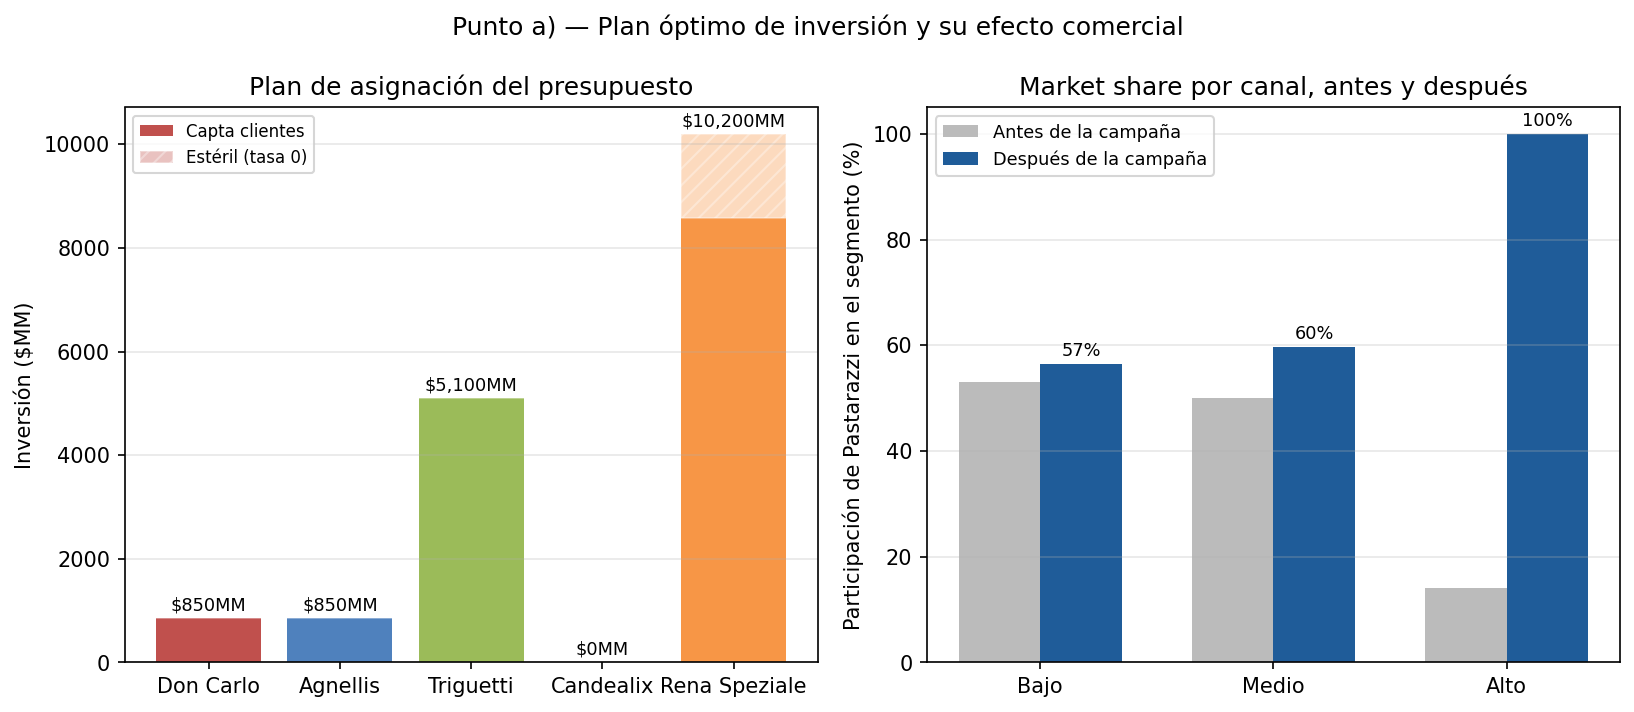
\includegraphics[width=0.82\linewidth]{../resultados/graficos/01_plan_base.png}
\caption{Plan óptimo de inversión (izquierda) y su efecto sobre la participación
de mercado por segmento (derecha). El segmento alto queda completamente saturado.}
\label{fig:plan_base}
\end{figure}

\begin{table}[htbp]
\centering\small
\caption{Mix comercial resultante (cifras en \$MM/año, salvo indicación).}
\begin{tabular}{lrrrrr}
\toprule
Marca & Inversión & Clientes nuevos & Fact. total & Utilidad neta & \% facturación \\
\midrule
\marca{doncarlo}{Don Carlo}  & 850     & 340.000   & 334.761   & 16.738,05 & 32{,}6\,\% \\
\marca{agnellis}{Agnellis}   & 850     & 425.000   & 210.051   & 15.753,82 & 20{,}5\,\% \\
\marca{triguetti}{Triguetti} & 5.100   & 1.020.000 & 245.208   & 22.068,72 & 23{,}9\,\% \\
\marca{candealix}{Candealix} & 0       & 0         &  78.600   &  6.288,00 &  7{,}7\,\% \\
\marca{rena}{Rena Speziale}  & 10.200  & 1.032.000 & 157.300   & 15.730,00 & 15{,}3\,\% \\
\midrule
\textbf{Total} & \textbf{17.000} & \textbf{2.817.000} & \textbf{1.025.920} & \textbf{76.578,60} & \textbf{100\,\%} \\
\bottomrule
\end{tabular}
\vspace{1mm}\\
\footnotesize Utilidad operativa: \$112.489,49\,MM. Market share: pasa de $48{,}10\,\%$ a $\mathbf{61{,}91\,\%}$.
\end{table}

\begin{table}[htbp]
\centering\small
\caption{Distribución por canal de venta (proxy: segmento de mercado, supuesto S9).}
\begin{tabular}{lrrrr}
\toprule
Segmento & Mercado (\$MM) & Share inicial & Share final & Cupo usado \\
\midrule
Bajo  & 881.500 & 53{,}0\,\% & 56{,}6\,\%  &  7{,}6\,\% \\
Medio & 614.800 & 50{,}0\,\% & 59{,}6\,\%  & 19{,}2\,\% \\
Alto  & 160.800 & 14{,}0\,\% & \textbf{100{,}0\,\%} & \textbf{100{,}0\,\%} \\
\bottomrule
\end{tabular}
\end{table}

El crecimiento se concentra casi todo en el segmento alto, que termina
completamente saturado; los segmentos bajo y medio apenas se tocan (usan
7,6\,\% y 19,2\,\% de su cupo disponible, respectivamente).

\paragraph{El hallazgo más importante del punto: se queman \$1.630\,MM sin
captar un solo cliente.} El segmento alto se llena por completo con
\$8.570\,MM invertidos en Rena Speziale (\$3.500\,MM al 150\,cl/\$MM más
\$5.070\,MM al 100\,cl/\$MM). Pero R4 exige
$x_{RS}\geq 2(x_{CAN}+x_{TRI})\geq 2\times 5.100=10.200$. Los
$10.200-8.570=1.630\,$MM que faltan hay que ponerlos igual —lo manda la
regla— aunque no exista ya ningún cliente premium por captar. Es casi el
$9,6\,\%$ de todo el presupuesto de la campaña, y es el argumento central de
la Consulta~4 (\S\ref{sec:consulta4}).

\begin{table}[htbp]
\centering\small
\caption{Estado de las restricciones activas y sus precios sombra.}
\label{tab:duales}
\begin{tabular}{llrr}
\toprule
Restricción & Descripción & Holgura & Precio sombra \\
\midrule
R1 & Presupuesto total & 0 (activa) & $+1{,}17875$ \\
R2 & Paridad Don Carlo = Agnellis & 0 (activa) & $-0{,}35875$ \\
R3 & Triguetti $\geq 30\,\%$ & 0 (activa) & $-2{,}49225$ \\
R4 & Rena $\geq 2(\text{Can}+\text{Tri})$ & 0 (activa) & $-1{,}17875$ \\
R5 & Tope $65\,\%$ gama baja & 1.815.000 & 0 \\
R10 (alto) & Saturación física del segmento alto & 0 (activa) & $+0{,}01340$ \\
\bottomrule
\end{tabular}
\end{table}

Cuatro de las once restricciones del modelo quedan activas, y entre ellas
consumen \$15.300\,MM de los \$17.000\,MM: \textbf{es el directorio, con sus
propias reglas, el que casi define el plan}, más que la optimización en sí.
El precio sombra de R1 ($+1{,}17875$) dice que cada millón adicional de
presupuesto valdría eso de utilidad extra —e iría, necesariamente, al par
Don Carlo/Agnellis, el único destino que queda libre. El de R3
($-2{,}49225$) es el más caro de todos, y se analiza en detalle en la
Consulta~4. R5, el techo del 65\,\% en la gama baja, no está activo: sobran
1.815.000 clientes de cupo, así que el freno del crecimiento en la gama baja
no es el mercado, es que las reglas del directorio no le dejan presupuesto.

\paragraph{Un resultado inesperado: los tres objetivos dan el mismo plan.}
Resolver con utilidad neta, utilidad operativa o facturación produce
\textbf{exactamente la misma asignación}: Don Carlo y Agnellis \$850\,MM cada
una, Triguetti \$5.100\,MM, Candealix \$0 y Rena Speziale \$10.200\,MM. No es
un error —se verificó a mano—: con R3 y R4 activas, la única plata que el
modelo puede repartir libremente son los \$1.700\,MM que sobran, y solo hay
dos destinos posibles para ponerlos (el par Don Carlo/Agnellis o Candealix); el
par gana en utilidad \emph{y} en facturación al mismo tiempo, así que no hay
nada que decidir entre los dos objetivos. La consecuencia para la discusión
del directorio es fuerte, y se retoma en la Consulta~3
(\S\ref{sec:consulta3}): bajo las reglas vigentes, la pelea entre accionistas
y directivos no tiene, en los hechos, nada para pelear.

% ============================================================================
\section{Análisis de sensibilidad}
\label{sec:sensibilidad}

\subsection{Rangos de nivel de actividad}
\label{sec:b1}

Esta sección lee los precios sombra y las holguras de la Tabla~\ref{tab:duales}
—en el sentido de la teoría de dualidad y sensibilidad de programación lineal
\cite{hillier}— como lo que son: el valor de relajar, o el costo de sostener,
cada regla del directorio.

\begin{itemize}
  \item \textbf{R1 (presupuesto).} Precio sombra $+1{,}17875$: pedirle al
  directorio un millón más de presupuesto vale eso de utilidad adicional. Es
  información directa y accionable para la Consulta~1.
  \item \textbf{R2 (paridad Don Carlo/Agnellis).} Precio sombra $-0{,}35875$:
  la regla cuesta plata porque obliga a poner en Don Carlo (que rinde 0,82 por
  \$MM) lo mismo que en Agnellis (que rinde 1,54). Es la cifra que sostiene
  numéricamente a la Consulta~2.
  \item \textbf{R3 (piso de Triguetti).} Precio sombra $-2{,}49225$, el más
  alto en valor absoluto del modelo. No es que Triguetti rinda mal —su primer
  tramo (1,044) casi empata con el par gama baja (1,179)—: lo caro es el
  arrastre que R4 le impone a Rena Speziale, tratado con todo detalle en la
  Consulta~4.
  \item \textbf{R4 (doble de Rena).} Precio sombra $-1{,}17875$: cada millón
  de más que R4 obliga a mandar a Rena por encima de lo que el segmento alto
  puede absorber es, directamente, un millón que no rinde nada.
  \item \textbf{R5 (tope del 65\,\% en gama baja).} Precio sombra $0$, con
  1.815.000 clientes de holgura: el techo comercial de la gama baja no está
  frenando nada hoy. Esto cambia si se relaja la paridad (Consulta~2): el
  barrido de esa sección muestra que R5 empieza a acercarse a activarse recién
  en escenarios extremos, aunque nunca llega a atar dentro del rango
  explorado.
\end{itemize}

Todos estos precios sombra valen \emph{dentro de un rango}: fuera de él, la
base óptima cambia y hay que resolver de nuevo, no extrapolar linealmente
—la advertencia central de la Clase 3 de la cátedra \cite{catedra-clases}—.
PuLP no devuelve esos rangos permisibles de manera directa —a diferencia del
informe de sensibilidad de Excel Solver—, así que se los calculó
re-resolviendo paramétricamente: barriendo el término independiente de cada
restricción y viendo en qué punto el precio sombra cambia de escalón. Es
exactamente el método que se usó para responder las Consultas~2, 3 y 4 (barrer
$k$, barrer $\varepsilon$, barrer el piso de Triguetti), y también para
mapear el límite exacto de R3: como se muestra en la
Sección~\ref{sec:consulta4}, la combinación de R3 y R4 dejan de tener solución
factible en conjunto apenas se supera el $33{,}33\,\%$ del presupuesto exigido
a Triguetti —un límite que se puede deducir algebraicamente, sin ni siquiera
correr el solver.

\subsection{Rangos de soluciones posibles}
\label{sec:b2}

Esta sección responde una pregunta distinta: no cuánto vale relajar una
restricción, sino cuánto se puede mover un \emph{coeficiente} del funcional
—un margen, una tasa de captación— antes de que cambie el plan óptimo. Es
particularmente relevante acá porque casi todos los coeficientes vienen de
estimaciones o de datos que el enunciado da con lenguaje aproximado
(``alrededor de'', ``cerca de''). Se corrió un barrido \emph{one-at-a-time}
(OAT) de $\pm30\,\%$ sobre cada supuesto numérico (S1 a S4, más R10, agregada
en el punto anterior), con todo lo demás fijo, y se resumió en un gráfico
tornado.

\begin{figure}[htbp]
\centering
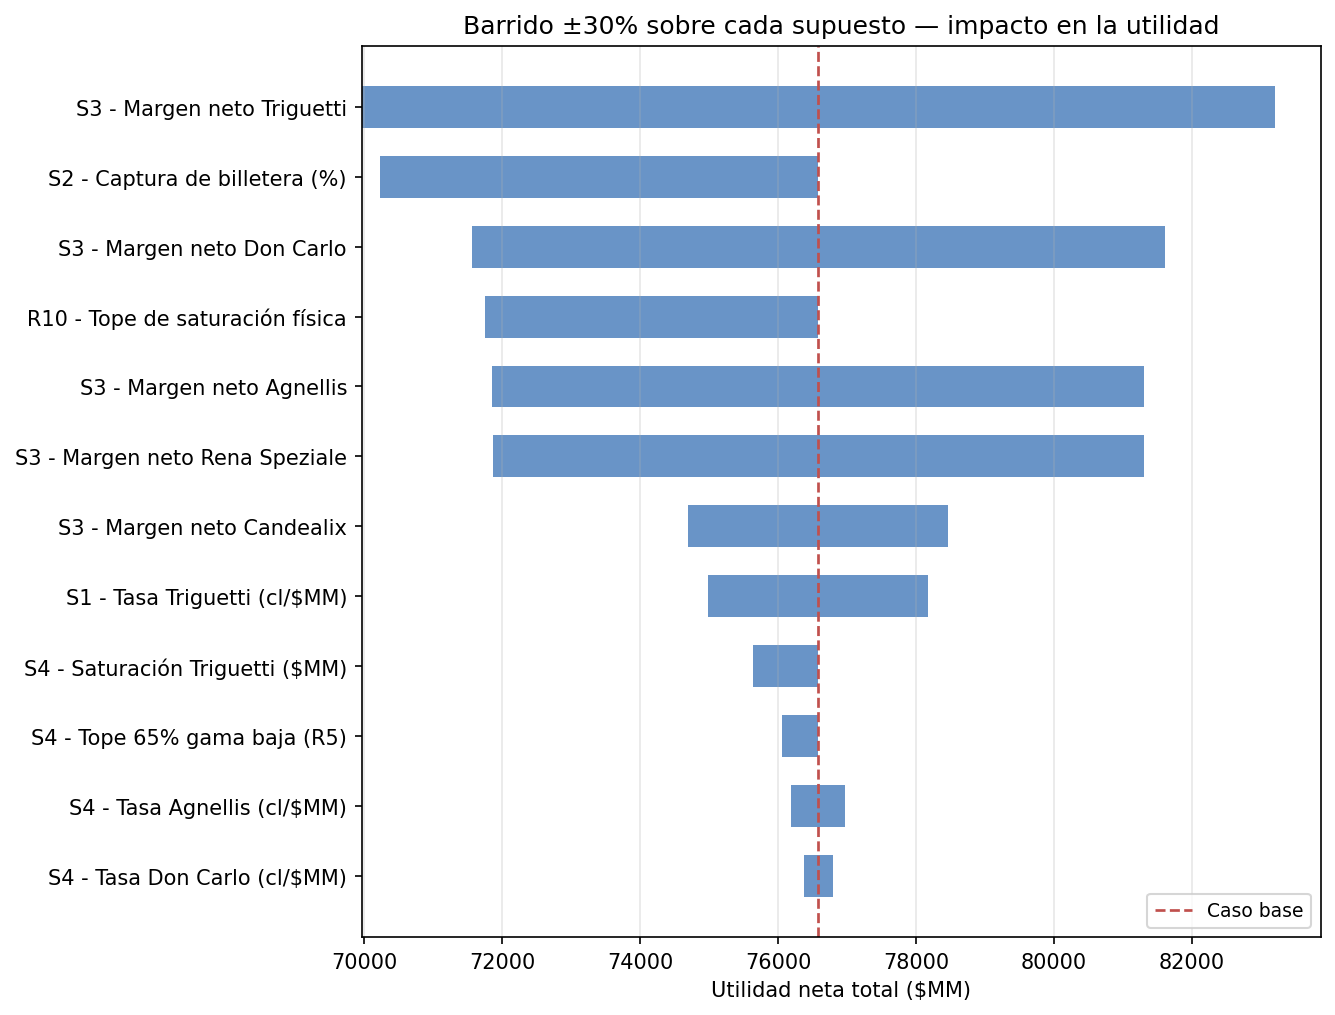
\includegraphics[width=0.72\linewidth]{../resultados/graficos/05_tornado_supuestos.png}
\caption{Barrido $\pm30\,\%$ sobre cada supuesto numérico. La línea punteada
marca la utilidad del caso base (\$76.578,60\,MM); el ancho de cada barra es
cuánto se mueve la utilidad en cada extremo del rango.}
\label{fig:tornado}
\end{figure}

\begin{table}[htbp]
\centering\small
\caption{Los seis parámetros que más mueven la utilidad (de 14 barridos).}
\begin{tabular}{lrrrc}
\toprule
Parámetro & $Z$ en $-30\,\%$ & $Z$ base & $Z$ en $+30\,\%$ & ¿Cambia el plan? \\
\midrule
S3 — margen neto Triguetti      & 69.957,98 & 76.578,60 & 83.199,21 & No \\
S2 — captura de billetera       & 70.231,47 & 76.578,60 & 76.578,60 & No \\
S3 — margen neto Don Carlo      & 71.557,18 & 76.578,60 & 81.600,01 & No \\
R10 — tope de saturación física & 71.754,60 & 76.578,60 & 76.578,60 & No \\
S3 — margen neto Agnellis       & 71.852,45 & 76.578,60 & 81.304,74 & No \\
S1 — tasa de Triguetti          & 74.981,27 & 76.578,60 & 78.175,91 & No \\
\bottomrule
\end{tabular}
\end{table}

La lectura es tranquilizadora para el plan del punto anterior:
\textbf{de los 14 parámetros barridos, uno solo cambia el plan óptimo} dentro
del rango de $\pm30\,\%$ —el tope del 65\,\% de la gama baja (R5), y solo en
su extremo inferior (55\,\%), un caso límite que se explica abajo—. Todos los
demás, incluido el que más mueve el nivel de la utilidad (el margen de
Triguetti, hasta $\pm 8{,}65\,\%$), dejan el reparto entre marcas intacto: lo
único que cambia es cuánto se gana, no en qué se invierte. Esto es exactamente
la clase de resultado que permite decir, en la Consulta~1, que el plan
propuesto no depende de forma frágil de los datos que tuvimos que completar
con criterio propio.

El caso de R5 merece una aclaración: el $-30\,\%$ teórico llevaría el tope al
$45{,}5\,\%$, un valor \textbf{por debajo del $53\,\%$ que Don Carlo y
Agnellis ya ocupan sin invertir un peso} —es decir, infactible por
construcción—. Se usó en su lugar $55\,\%$ como el extremo inferior
plausible, y ahí sí el plan cambia levemente: es la señal de que el
verdadero ``piso'' de esta regla no es un $-30\,\%$ cualquiera, sino
exactamente el share ya instalado.

\paragraph{Escenarios estructurales.} Además de los parámetros numéricos, se
resolvió el modelo completo bajo lecturas alternativas de los supuestos que no
son números sino decisiones de interpretación (S5, S7 y S8).

\begin{table}[htbp]
\centering\small
\caption{Escenarios estructurales: mismo modelo, otra lectura del supuesto.}
\begin{tabular}{p{6.6cm}rrc}
\toprule
Escenario & $Z$ (\$MM) & $\Delta Z$ vs. base & ¿Cambia el plan? \\
\midrule
Base (todas las lecturas adoptadas) & 76.578,60 & — & — \\
S5 — captación repartida según mix Fig.~2 & 76.967,99 & $+0{,}51\,\%$ & No \\
S7a — R3 sobre lo asignado, en vez de sobre \$17.000\,MM & 76.578,60 & $0{,}00\,\%$ & No \\
S7b — R4 como igualdad en vez de piso & 76.578,60 & $0{,}00\,\%$ & No \\
S8 — descontando el presupuesto del funcional & 59.578,60 & $-22{,}20\,\%$ & No$^{*}$ \\
\bottomrule
\end{tabular}
\vspace{1mm}\\
\footnotesize $^*$El plan óptimo es idéntico; solo cambia el número que se
reporta como utilidad ($Z-\$17.000\,\text{MM}$).
\end{table}

Ninguno de estos cuatro cambios de interpretación mueve el plan óptimo. La
lectura alternativa de S5 (repartir la captación de cada marca según el mix
normalizado de la Fig.~2 en lugar de asignarla entera a su segmento de
posicionamiento) sube la utilidad apenas medio punto porcentual: aunque es,
en teoría, el supuesto que más resultados toca (Tabla~\ref{tab:mapa_supuestos}),
en la práctica el plan óptimo es tan parecido bajo una lectura como bajo la
otra porque las restricciones activas (R3, R4) siguen fijando casi todo el
presupuesto de antemano. S7a y S7b directamente no mueven nada, porque en el
óptimo el presupuesto se agota siempre (así que ``30\,\% de lo asignado''
coincide con ``30\,\% del total'') y R4 ya se cumplía con holgura cero (así
que exigirlo como igualdad no quita nada). Y S8 confirma lo que ya se había
anticipado: descontar el presupuesto del funcional es solo un cambio de
presentación del número, no del plan. Por último, R6 —el umbral de
producción de Candealix— tampoco se activa en ninguno de estos escenarios,
porque ninguno modifica la facturación \emph{base} de la marca, que ya supera
el umbral 17,5 veces sin necesidad de invertir un peso.

% ============================================================================
\section{Representación gráfica del proceso}

El esquema de la Figura~\ref{fig:proceso} resume, de punta a punta, cómo el
presupuesto de marketing se transforma en utilidad: la plata se reparte entre
las cinco marcas, cada una capta clientes nuevos en su segmento a una tasa que
depende de cuánto ya se invirtió, esos clientes nuevos facturan según el gasto
anual de su segmento, y la facturación por el margen da la utilidad. Las
reglas del directorio (R2, R3, R4) atraviesan ese flujo imponiendo relaciones
fijas entre ramas que, de otro modo, el modelo repartiría con total libertad;
R5 y R10 actúan como topes de capacidad sobre lo que cada segmento puede
todavía absorber.

\begin{figure}[htbp]
\centering
\resizebox{\linewidth}{!}{%
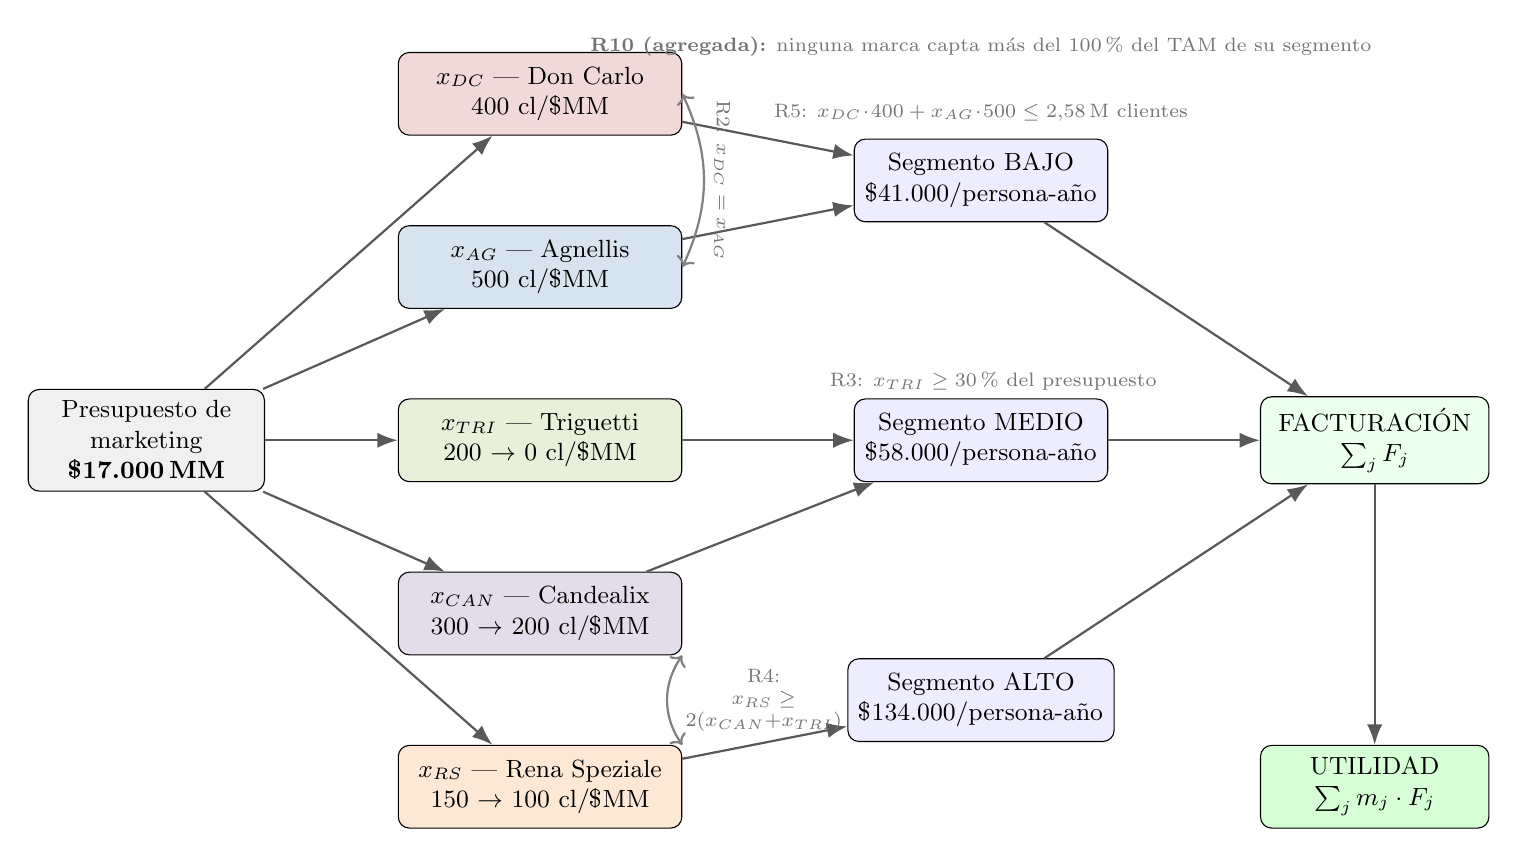
\begin{tikzpicture}[
  box/.style={draw, rounded corners, align=center, minimum height=1.05cm, font=\small, inner sep=4pt},
  arrow/.style={-{Latex[length=2.6mm]}, thick, color=black!65},
  tag/.style={font=\scriptsize, align=center, text=black!55}
]

\node[box, minimum width=3.0cm, fill=black!6] (pres) at (0,0)
  {Presupuesto de\\marketing\\\textbf{\$17.000\,MM}};

\node[box, minimum width=3.6cm, fill=doncarlo!22] (dc)  at (5.0, 4.4) {$x_{DC}$ — Don Carlo\\400 cl/\$MM};
\node[box, minimum width=3.6cm, fill=agnellis!22] (ag)  at (5.0, 2.2) {$x_{AG}$ — Agnellis\\500 cl/\$MM};
\node[box, minimum width=3.6cm, fill=triguetti!22](tri) at (5.0, 0.0) {$x_{TRI}$ — Triguetti\\200 $\to$ 0 cl/\$MM};
\node[box, minimum width=3.6cm, fill=candealix!22](can) at (5.0,-2.2) {$x_{CAN}$ — Candealix\\300 $\to$ 200 cl/\$MM};
\node[box, minimum width=3.6cm, fill=rena!22]     (rs)  at (5.0,-4.4) {$x_{RS}$ — Rena Speziale\\150 $\to$ 100 cl/\$MM};

\draw[arrow] (pres) -- (dc);
\draw[arrow] (pres) -- (ag);
\draw[arrow] (pres) -- (tri);
\draw[arrow] (pres) -- (can);
\draw[arrow] (pres) -- (rs);

\node[box, minimum width=3.2cm, fill=blue!7] (bajo)  at (10.6, 3.3) {Segmento BAJO\\\$41.000/persona-año};
\node[box, minimum width=3.2cm, fill=blue!7] (medio) at (10.6, 0.0) {Segmento MEDIO\\\$58.000/persona-año};
\node[box, minimum width=3.2cm, fill=blue!7] (alto)  at (10.6,-3.3) {Segmento ALTO\\\$134.000/persona-año};

\draw[arrow] (dc)  -- (bajo);
\draw[arrow] (ag)  -- (bajo);
\draw[arrow] (tri) -- (medio);
\draw[arrow] (can) -- (medio);
\draw[arrow] (rs)  -- (alto);

\node[box, minimum width=2.9cm, fill=green!7] (fact) at (15.6, 0.0) {FACTURACIÓN\\$\sum_j F_j$};
\node[box, minimum width=2.9cm, fill=green!16] (util) at (15.6,-4.4) {UTILIDAD\\$\sum_j m_j \cdot F_j$};

\draw[arrow] (bajo)  -- (fact);
\draw[arrow] (medio) -- (fact);
\draw[arrow] (alto)  -- (fact);
\draw[arrow] (fact)  -- (util);

% --- reglas del directorio -------------------------------------------------
\draw[<->, thick, black!50] (dc.east) to[bend left=25] node[tag, above, sloped] {R2: $x_{DC}=x_{AG}$} (ag.east);

\node[tag, right=2mm of tri, xshift=1.55cm, yshift=0.75cm, align=left] {R3: $x_{TRI}\geq 30\,\%$ del presupuesto};

\draw[<->, thick, black!50] (can.south east) to[bend right=35] node[tag, right, xshift=1mm] {R4:\\$x_{RS}\geq$\\$2(x_{CAN}{+}x_{TRI})$} (rs.north east);

\node[tag, above=1mm of bajo, align=center] {R5: $x_{DC}\!\cdot\!400+x_{AG}\!\cdot\!500 \leq 2{,}58\,\text{M clientes}$};
\node[tag] at (10.6, 5.0) {\textbf{R10 (agregada):} ninguna marca capta más del 100\,\% del TAM de su segmento};

\end{tikzpicture}}
\caption{Esquema del proceso: del presupuesto de marketing a la utilidad, marca
por marca y segmento por segmento. Las flechas curvas señalan las reglas del
directorio que atan la inversión entre marcas.}
\label{fig:proceso}
\end{figure}

% ============================================================================
\section{Librerías utilizadas}
\label{sec:librerias}

Todo el trabajo se hizo en \textbf{Python 3.10}, con el siguiente stack:

\begin{itemize}
  \item \textbf{PuLP} \cite{pulp} (solver \textbf{CBC} \cite{cbc}): modelado
  y resolución del problema de programación lineal. Se prefirió por sobre
  \texttt{scipy.optimize.linprog} —sugerido también en los links de la
  consigna \cite{consigna}— porque PuLP permite nombrar cada restricción y
  leer después, por nombre, su precio sombra (\texttt{.pi}) y su holgura
  (\texttt{.slack}); con \texttt{scipy} eso exige trabajar directamente con
  matrices e índices, que es más incómodo cuando el modelo tiene once
  restricciones con nombre propio.
  \item \textbf{pandas}: construcción de las tablas de datos derivados y de
  resultados.
  \item \textbf{matplotlib}: los cinco gráficos de resultados del informe (el
  esquema del proceso de la Figura~\ref{fig:proceso} está hecho con Ti\emph{k}Z).
\end{itemize}

Todo el modelo se escribió \textbf{una sola vez}, como una función
parametrizada,
\begin{quote}
\centering\small\texttt{modelo.resolver(params, objetivo, epsilon, desactivar)}
\end{quote}
que sirve tanto para el caso base como para los más de setenta escenarios que
se corrieron en total entre los barridos de sensibilidad y las cuatro
consultas: nunca se copió el modelo para responder una pregunta distinta,
siempre se llamó a la misma función con otros parámetros.

Una limitación conocida de PuLP, a diferencia del informe de sensibilidad de
Excel Solver o de LINDO, es que no devuelve directamente los rangos
permisibles de las restricciones ni de los coeficientes del funcional. Se
resolvió recalculándolos de forma paramétrica: re-resolviendo el modelo en una
grilla de valores y detectando en qué punto el precio sombra cambia de
escalón. Es, en esencia, el gráfico de ``RHS Parametrics'' que se ve en la
teoría de la materia, hecho a mano con el propio solver.

Como control de calidad del código, se armaron tres capas de verificación
automática que corren antes de aceptar cualquier resultado: 31 asserts sobre
los datos derivados (mercado, facturación base, coeficientes del funcional),
un conjunto de cotas deducidas a mano sobre el óptimo de cada corrida, y la
reconstrucción manual —con aritmética simple— de los cinco precios sombra no
nulos del caso base, que coinciden con lo que devuelve el solver hasta la
quinta cifra decimal.

% ============================================================================
\section{Respuestas a las consultas del directorio}

Esta sección responde, en orden, las cuatro consultas concretas de la página 4
de la consigna, apoyándose en el modelo y en el análisis de sensibilidad ya
desarrollados.

\subsection{Consulta 1 — El plan de asignación del presupuesto}

El plan que equilibra captación de clientes y rentabilidad es el que se
presentó en la Sección~\ref{sec:resolucion}: \textbf{Don Carlo \$850\,MM,
Agnellis \$850\,MM, Triguetti \$5.100\,MM, Candealix \$0 y Rena Speziale
\$10.200\,MM}, con una utilidad neta de \$76.578,60\,MM y un market share que
pasa del $48{,}10\,\%$ al $61{,}91\,\%$.

El mix resultante está dominado, en términos de facturación, por Triguetti
(23,9\,\%) y Don Carlo (32,6\,\%), pero en términos de \emph{crecimiento}
relativo el protagonista es otro: Rena Speziale crece un $727\,\%$ sobre su
base (contra $4$--$32\,\%$ del resto), porque partía de una base instalada
minúscula (apenas \$19.012\,MM) y recibe, por las reglas R3+R4, más plata de
la que su segmento puede absorber de forma eficiente. La distribución por
canal (Tabla del \S\ref{sec:resolucion}) muestra que casi todo ese crecimiento
se concentra en el segmento alto, que termina saturado al $100\,\%$, mientras
que el bajo y el medio apenas se mueven.

\textbf{Candealix queda directamente fuera del plan}, pese a ser rentable por
sí sola (1,392 de utilidad por \$MM, mejor que Don Carlo). La razón no es su
propio rendimiento: es que, por R4, cada peso que recibiría arrastraría dos
pesos adicionales y obligatorios hacia Rena Speziale, que ya está saturada.
Su costo efectivo, contando ese arrastre, es de apenas 0,464 por \$MM —menos
de la mitad de lo que rinde el par de la gama baja—, así que el modelo
directamente no le asigna nada.

El hallazgo que más conviene destacarle al directorio es el de la
Sección~\ref{sec:resolucion}: sus propias reglas obligan a quemar
\$1.630\,MM —casi uno de cada diez pesos del presupuesto— sin captar un solo
cliente adicional, porque exigen más plata para Rena Speziale de la que su
segmento, ya saturado, puede absorber.

\subsection{Consulta 2 — Escenarios de crecimiento de Agnellis}
\label{sec:consulta2}

La regla de paridad (R2, supuesto S6) se generalizó de $x_{DC}=x_{AG}$ a
$x_{DC}=k\cdot x_{AG}$, y se barrió $k$ desde $1{,}00$ (el caso base) hasta
$0{,}00$ (toda la plata libre del par gama baja va a Agnellis), reutilizando
el mismo modelo sin tocar una línea de código.

\begin{table}[htbp]
\centering\small
\caption{Barrido de la paridad Don Carlo/Agnellis.}
\begin{tabular}{rrrrr}
\toprule
$k$ & Don Carlo (\$MM) & Agnellis (\$MM) & Presencia DC$^{*}$ & Utilidad neta (\$MM) \\
\midrule
1,00 (base) & 850,00 & 850,00   & 64{,}68\,\% & 76.578,60 \\
0,75        & 728,57 & 971,43   & 64{,}22\,\% & 76.665,72 \\
0,50        & 566,67 & 1.133,33 & 63{,}60\,\% & 76.781,89 \\
0,30        & 392,31 & 1.307,69 & 62{,}94\,\% & 76.906,99 \\
0,00        & 0,00   & 1.700,00 & 61{,}45\,\% & 77.188,47 \\
\bottomrule
\end{tabular}
\vspace{1mm}\\
\footnotesize$^{*}$Presencia de Don Carlo dentro del par, medida sobre el
mercado real (base instalada + campaña).
\end{table}

\begin{figure}[htbp]
\centering
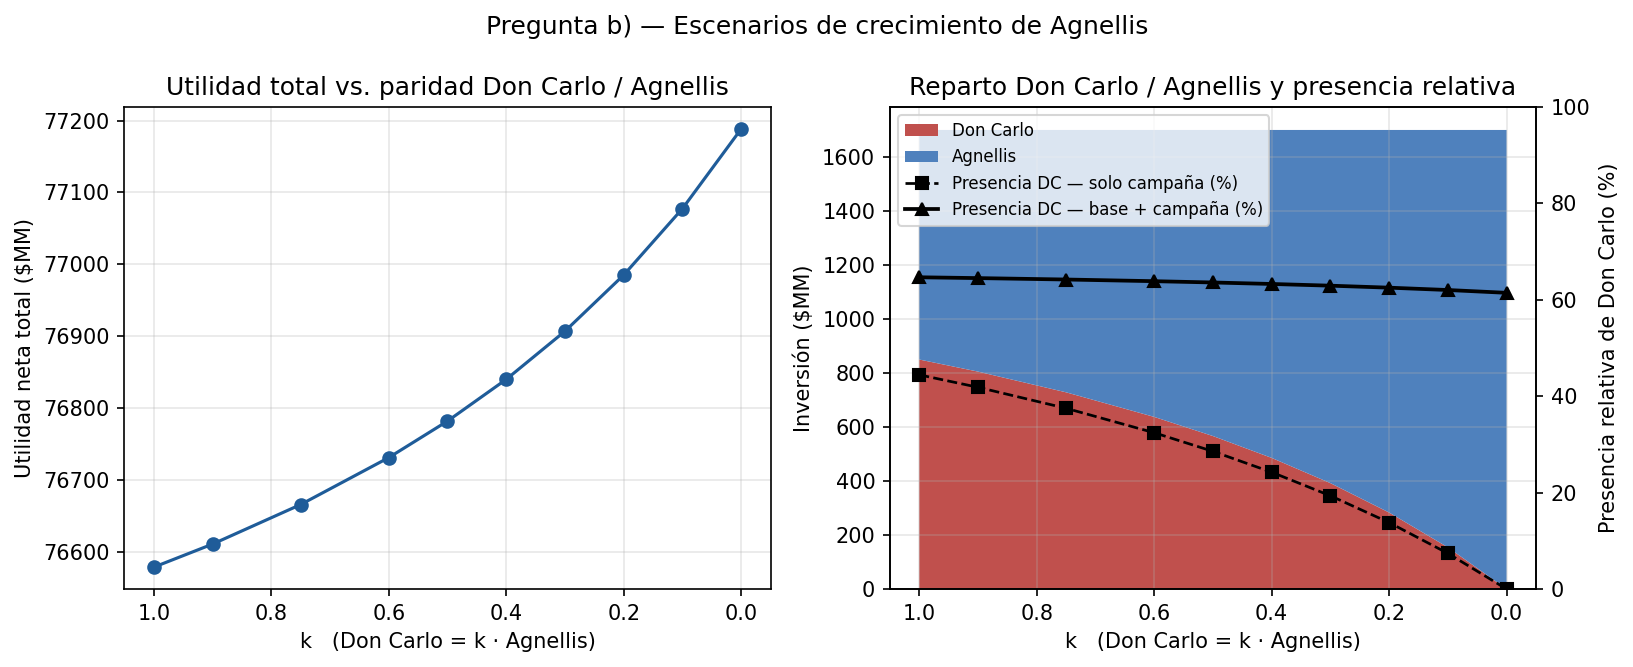
\includegraphics[width=0.8\linewidth]{../resultados/graficos/02_utilidad_vs_k_paridad.png}
\caption{Izquierda: utilidad total según la paridad. Derecha: reparto del
presupuesto y las dos formas de medir la presencia de Don Carlo.}
\label{fig:pregunta_b}
\end{figure}

Antes de contestar, conviene aclarar algo que la primera versión de este
análisis pasó por alto: \textbf{``presencia'' se puede medir de dos formas muy
distintas}, y según cuál se use la respuesta cambia por completo. Medida solo
entre los clientes que la campaña de este año capta, la presencia de Don Carlo
cae del $44{,}44\,\%$ al $0\,\%$ —una caída total—. Pero Don Carlo ya tiene
7.525.000 clientes de base instalada, y la campaña entera mueve apenas
340.000 (el 4,5\,\% de esa base): medida sobre el mercado real, la presencia de
Don Carlo pasa de $64{,}68\,\%$ a $61{,}45\,\%$, una caída de apenas
\textbf{3,2 puntos}. La segunda métrica es la que realmente responde lo que el
enunciado pregunta: la de un consumidor evaluando qué marca de gama baja
sigue siendo la líder, no la de contar solamente lo que se vendió \emph{este}
año.

Con esa aclaración, las dos preguntas del enunciado tienen respuesta directa:

\begin{itemize}
  \item \textbf{¿Cuánto necesita invertir Don Carlo para no perder presencia
  significativa?} Prácticamente nada. Aun en el escenario extremo donde no
  recibe un solo peso ($k=0$), Don Carlo sigue siendo la marca dominante de la
  gama baja, con solo 3,2 puntos menos de presencia relativa. Si de todos
  modos se quiere sostener la presencia \emph{dentro} de la campaña —por
  ejemplo, para no ceder terreno mes a mes en la conversación con el canal—,
  la relación es una hipérbola ($400k/(400k+500)$, no lineal), y con
  $k\approx 0{,}5$--$0{,}6$ Don Carlo retiene entre el 64\,\% y el 73\,\% de
  su presencia original dentro de la campaña.
  \item \textbf{¿Qué efecto tiene esto en la utilidad total?} Positivo pero
  chico: soltar la paridad por completo suma apenas \$609,88\,MM
  ($+0{,}80\,\%$). Es coherente con el precio sombra de R2 en el caso base
  ($-0{,}35875$): la paridad es barata de sostener porque Don Carlo (0,82) y
  Agnellis (1,5375) no son tan distintos entre sí como el resto de las marcas
  del portafolio.
\end{itemize}

En síntesis: con estos números, la decisión de soltar o no la paridad no es
realmente una decisión económica —lo que está en juego es menos de un punto de
utilidad—, sino una decisión sobre cuánto arriesgo comercial de imagen se
quiere tomar a cambio de casi nada.

\subsection{Consulta 3 — Crecimiento de market share vs. crecimiento en rentabilidad}
\label{sec:consulta3}

El plan original preveía aplicar el método $\varepsilon$-constraint
directamente sobre el caso base (maximizar utilidad sujeto a un piso de
facturación, barriendo ese piso) para trazar la frontera de Pareto entre
utilidad y participación. Pero el propio punto anterior ya había mostrado algo
importante: bajo las reglas vigentes, \textbf{los tres objetivos posibles dan
el mismo plan óptimo} (\S\ref{sec:resolucion}). Eso significa que la frontera,
tal como está planteado el problema hoy, colapsa en un único punto: no hay
nada que barrer.

Eso no invalida la pregunta, la reformula: si el directorio quiere entender su
margen de maniobra entre rentabilidad y participación, primero tiene que saber
que \textbf{hoy no tiene ninguno}, y recién después preguntarse cuánto
aparecería si se relajaran sus propias reglas. Por eso el barrido se corrió en
cuatro escenarios: las reglas vigentes, sin R3, sin R4, y sin ninguna de las
dos.

\begin{table}[htbp]
\centering\small
\caption{Cuánto trade-off aparece en cada escenario (recordar: 1 punto de
share equivale a \$16.571\,MM de facturación).}
\begin{tabular}{lrrrr}
\toprule
Escenario & Share mín.--máx. & Puntos en juego & Utilidad máx. & Costo medio/punto \\
\midrule
Reglas actuales   & $61{,}91\,\%$ (fijo)     & 0{,}00 & 76.578,60 & — \\
Sin R3            & $65{,}56$--$65{,}92\,\%$ & 0{,}36 & 80.100,96 & \$796\,MM \\
Sin R4            & $63{,}92$--$65{,}10\,\%$ & 1{,}18 & 79.296,92 & \$883\,MM \\
Sin R3 ni R4      & $65{,}52$--$66{,}22\,\%$ & 0{,}70 & 80.253,43 & \$529\,MM \\
\bottomrule
\end{tabular}
\end{table}

\begin{figure}[htbp]
\centering
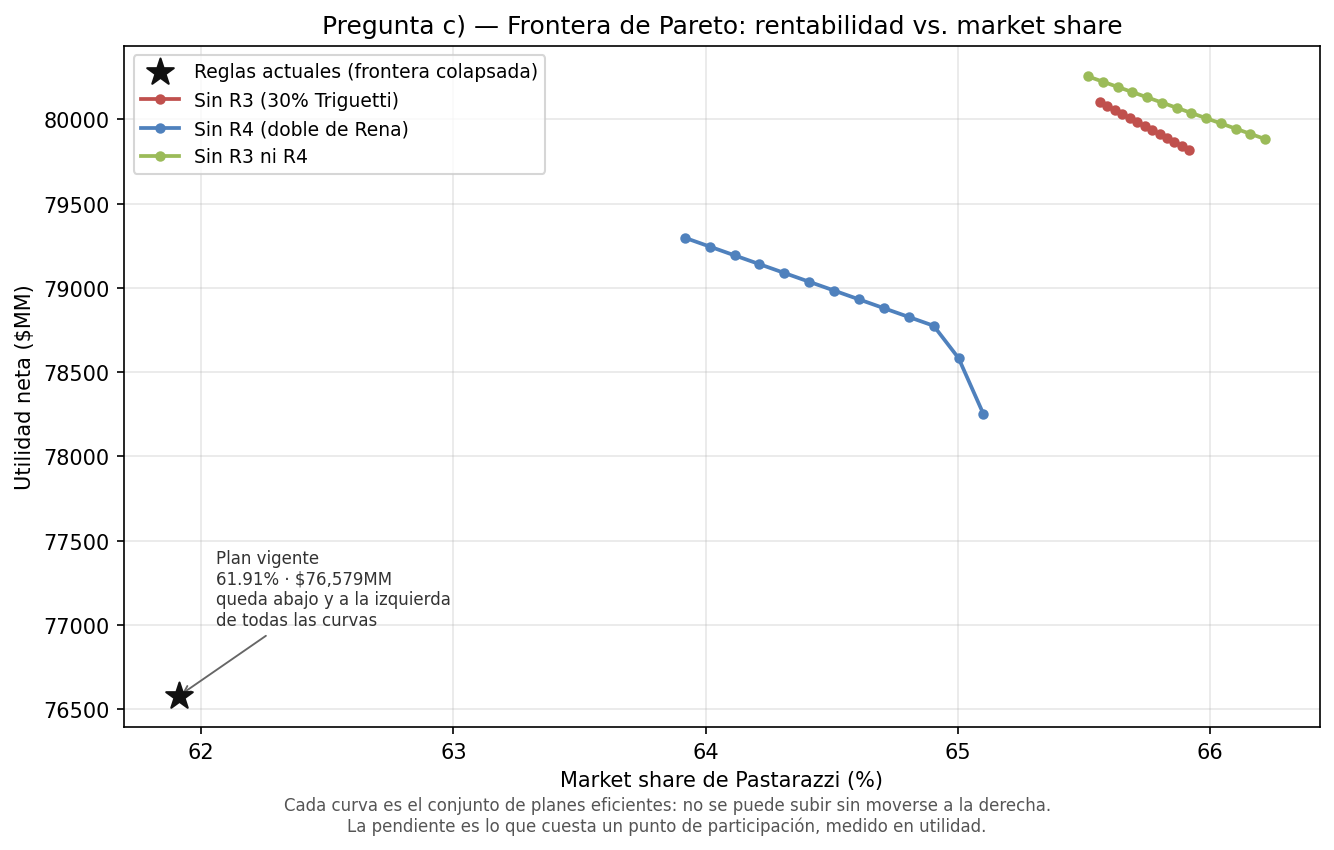
\includegraphics[width=0.72\linewidth]{../resultados/graficos/03_frontera_pareto.png}
\caption{Frontera de Pareto entre utilidad y market share, en los cuatro
escenarios. El plan vigente es un punto suelto: no hay curva que recorrer.}
\label{fig:pareto}
\end{figure}

Tres lecturas se desprenden de este barrido:

\begin{enumerate}
  \item \textbf{Hoy no hay ninguna discusión que resolver.} Accionistas y
  directivos quieren cosas distintas, pero con las reglas actuales el plan
  óptimo es el mismo para los dos: R3 y R4 ya consumen \$15.300\,MM de los
  \$17.000\,MM y no dejan margen de decisión real.
  \item \textbf{El plan vigente no es una elección prudente, está dominado.}
  En el gráfico, el punto del plan actual queda abajo y a la izquierda de las
  tres curvas: los tres escenarios relajados le ganan \emph{en las dos
  dimensiones a la vez}. Pasar a ``sin R3 ni R4'' sumaría 3,6 puntos de share
  \emph{y} \$3.675\,MM de utilidad, simultáneamente. No es que las reglas del
  directorio compren participación a costa de rentabilidad, ni al revés:
  están dejando las dos cosas sobre la mesa.
  \item \textbf{El precio del share no es constante.} En el escenario ``sin
  R4'' el costo marginal de un punto adicional arranca en \$529\,MM y termina
  en \$3.365\,MM —un salto de 6,4 veces—: los primeros puntos de
  participación se compran barato reasignando presupuesto entre marcas, pero
  los últimos exigen empujar a Rena Speziale contra el techo, ya saturado, del
  segmento alto.
\end{enumerate}

La traducción para el directorio es esta: \textbf{el problema no es
rentabilidad contra participación, es que las propias reglas del directorio
le impiden a la empresa tener las dos cosas a la vez}. La pelea entre
accionistas y directivos no se resuelve eligiendo un objetivo por sobre el
otro —bajo las reglas actuales da lo mismo—, se resuelve revisando esas
reglas. Y aun así conviene bajar la expectativa sobre lo que queda para
discutir después: liberando ambas restricciones, el margen de negociación
real es de apenas \textbf{0,70 puntos} de participación, y aun en el escenario
más favorable de los tres (sin R4) no supera los \textbf{1,18 puntos}. Es
decir: lo grande está en revisar las reglas —3,6 puntos de participación y
\$3.675\,MM de utilidad, sin resignar nada a cambio—, no en la negociación que
viene después.

\subsection{Consulta 4 — ¿Está mal la regla del 30\,\% obligatorio en Triguetti?}
\label{sec:consulta4}

El precio sombra de R3 en el caso base ($-2{,}49225$ por \$MM forzado) sugiere
que la regla sale cara. Pero atribuirle ese costo a Triguetti sería una
lectura apurada: el primer tramo de Triguetti rinde 1,044 por \$MM, casi lo
mismo que el par gama baja (1,179), el destino alternativo de esa plata. La
descomposición a mano del precio sombra separa los dos efectos:

\[
\begin{aligned}
&\underbrace{(1{,}044 - 1{,}179)}_{\text{(a) efecto directo: Triguetti vs. el par}} \; + \;
\underbrace{2\times(-1{,}179)}_{\text{(b) efecto arrastre: 2 \$MM extra a Rena, por R4}} \\[4pt]
&\;=\; -0{,}135 - 2{,}358 \;=\; -2{,}492
\end{aligned}
\]

De los \$2,49 de costo por millón forzado, \textbf{solo \$0,13 salen de
Triguetti en sí}; los \$2,36 restantes —el $95\,\%$ del costo total— vienen
de que R4 encadena a Rena Speziale al tamaño de Triguetti, y Rena ya está
saturada. El problema no es Triguetti, es la combinación de las dos reglas.

\begin{table}[htbp]
\centering\small
\caption{Barrido del piso mínimo exigido a Triguetti.}
\begin{tabular}{rrrrr}
\toprule
Piso mínimo & Triguetti (\$MM) & Rena (\$MM) & Inv. estéril (\$MM) & Utilidad neta (\$MM) \\
\midrule
0\,\%        & 0     & 8.570  & 0     & 80.100,96 \\
10\,\%       & 1.700 & 8.570  & 0     & 79.509,36 \\
20\,\%       & 3.400 & 8.570  & 0     & 78.917,76 \\
30\,\% (base)& 5.100 & 10.200 & 1.630 & 76.578,60 \\
\bottomrule
\end{tabular}
\end{table}

\begin{figure}[htbp]
\centering
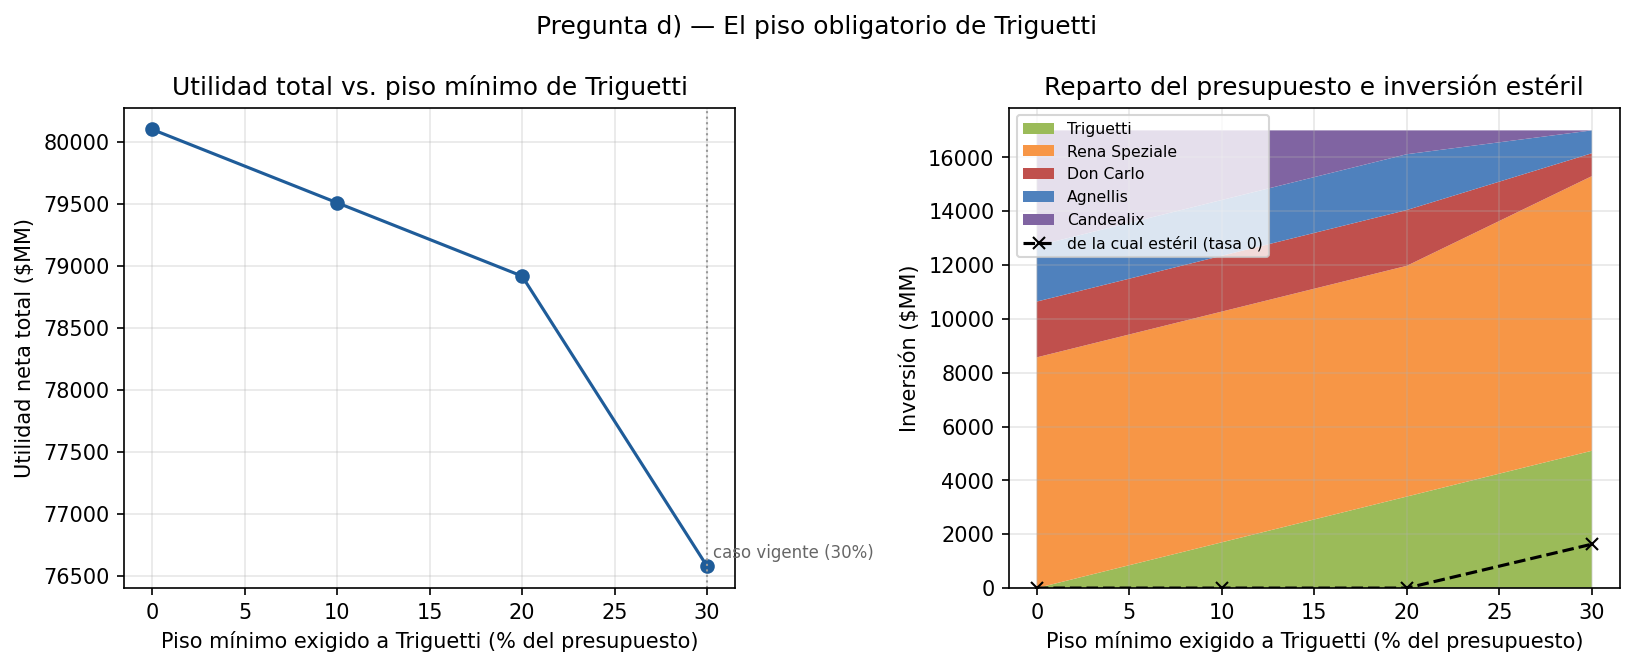
\includegraphics[width=0.8\linewidth]{../resultados/graficos/04_utilidad_vs_pct_triguetti.png}
\caption{Utilidad total (izquierda) y reparto del presupuesto (derecha) según
el piso mínimo exigido a Triguetti. La inversión estéril recién aparece a
partir del 30\,\%.}
\label{fig:pregunta_d}
\end{figure}

Un dato llamativo del propio barrido: mientras el piso está en $10\,\%$ o
$20\,\%$, Rena Speziale se queda en \$8.570\,MM —el óptimo que satura su
segmento sin que R4 llegue a atar— y es Candealix, no Rena, la que absorbe el
resto del presupuesto libre. R4 solo empieza a atar, y a arrastrar plata
estéril hacia Rena, a partir del $30\,\%$. Bajar la regla de Triguetti al
$20\,\%$, por ejemplo, no solo ahorraría el costo directo: eliminaría por
completo la inversión estéril.

\textbf{Un hallazgo adicional, más contundente todavía: subir el piso de
Triguetti al 40\,\% no da un plan peor, da directamente un modelo sin
solución.} Con Candealix en su mínimo, R3 y R4 juntas exigen
$x_{TRI}+x_{RS}\geq 3\,x_{TRI}\geq 3\times(\text{piso})$; para que eso quepa
en el presupuesto hace falta $\text{piso}\leq 1/3=33{,}33\,\%$. La regla
vigente del $30\,\%$ ya está a apenas 3,3 puntos porcentuales de volver
\emph{imposible} cumplir las dos reglas del directorio al mismo tiempo, sin
que exista ningún plan de ningún tipo que las satisfaga a la vez.

Este resultado se sostiene, además, en todo el rango plausible del supuesto
S1 (la tasa de captación de Triguetti que el enunciado no da): repitiendo el
barrido con la tasa en 140, 200 y 260 clientes por \$MM, el costo de la regla
se mueve entre \$1.925\,MM y \$5.120\,MM, mostrando la misma estructura en
los tres casos —no depende del dato que faltaba.

\paragraph{Entonces, ¿tiene razón el gerente?} En el número, sí: la regla del
$30\,\%$ le cuesta a la empresa del orden de \$3.522\,MM al año
($+4{,}6\,\%$ de utilidad si se elimina por completo), y de paso obliga a
quemar \$1.630\,MM sin captar un cliente. Pero el diagnóstico del gerente
apunta al lugar equivocado: la culpa no es de Triguetti, que rinde casi lo
mismo que el resto del portafolio, sino de la regla del doble para Rena
Speziale, que la ata a un segmento premium ya saturado. Y hay una salvedad
más de fondo, que ningún número del modelo puede resolver por sí solo: este
modelo optimiza \emph{un año}. Lo que la regla del 30\,\% protege —identidad
de marca, presencia constante en góndola, poder de negociación con
supermercados y almacenes— no está representado en el funcional. La
respuesta que este análisis puede dar con responsabilidad no es ``sacar la
regla'', sino: \emph{la regla cuesta \$3.522\,MM al año; que el directorio
decida, con ese número sobre la mesa, si la presencia de marca que compra vale
más que esa plata}. Eso es un aporte de análisis; discutir si el gerente
``tiene razón'' sin ese número sería solo una opinión.

% ============================================================================
\section{Conclusiones generales}

El modelo de programación lineal armado para Pastarazzi arroja un resultado
que probablemente no es el que el directorio esperaba: \textbf{sus propias
reglas de asignación —la paridad de Don Carlo y Agnellis, el piso de
Triguetti y el doble de Rena Speziale— dejan tan poco margen de maniobra que
terminan decidiendo casi todo el plan por sí solas}, antes de que la
optimización entre a jugar. De los \$17.000\,MM del presupuesto, \$15.300\,MM
quedan comprometidos de antemano por esas tres reglas, y una fracción no
menor de esa plata —\$1.630\,MM, casi el 10\,\%— se termina invirtiendo sin
captar un solo cliente nuevo, porque las reglas empujan más presupuesto hacia
Rena Speziale del que su segmento, ya saturado, puede absorber.

Esa rigidez tiene una consecuencia que atraviesa buena parte de este informe:
la discusión entre accionistas (que quieren rentabilidad) y directivos (que
quieren facturación) es, tal como está planteado el problema hoy, una
discusión sin objeto —los tres objetivos posibles dan exactamente el mismo
plan—. El conflicto solo se vuelve real, y se puede empezar a cuantificar en
plata y en puntos de participación, cuando se relajan las reglas que el propio
directorio impuso.

El análisis de sensibilidad, por su parte, deja una conclusión tranquilizadora
sobre la robustez del trabajo: de los catorce parámetros que tuvimos que
completar o estimar porque el enunciado no los daba con precisión, solo uno
—y en un caso límite— altera el plan óptimo dentro de un rango de variación
razonable ($\pm30\,\%$). El plan del punto 1 no depende de haber adivinado
bien un número: depende, sobre todo, de las reglas del directorio, que están
dadas y no admiten ambigüedad.

Por último, el ejercicio de completar el modelo con supuestos propios —en
particular, la restricción R10 de saturación física, que no está en el
enunciado pero sin la cual el modelo predice vender pastas a más gente de la
que existe— confirma algo que vale la pena remarcar: un modelo de
programación lineal no es solamente una cuenta, es una traducción de un
problema real a números, y esa traducción exige criterio, chequeo y, cuando
hace falta, la humildad de encontrar un resultado imposible y corregirlo antes
de confiar en lo que el solver devuelve.

% ============================================================================
\renewcommand{\refname}{Bibliografía}
\addcontentsline{toc}{section}{Bibliografía}

\begin{thebibliography}{9}

\bibitem{hillier} Hillier, F. S. y Lieberman, G. J. (2015).
  \emph{Introducción a la Investigación de Operaciones} (9.\textsuperscript{a}
  ed.). México: McGraw-Hill Interamericana. Capítulos 1 y 3 (formulación y
  resolución de modelos de programación lineal) y Capítulo 6 (teoría de la
  dualidad y análisis de sensibilidad).

\bibitem{catedra-clases} Cátedra de Optimización, UCA
  (2026). \emph{Clase 1 — Introducción}, \emph{Clase 2 — Formulación general}
  y \emph{Clase 3 — Análisis de sensibilidad}. Material de cátedra, 2.\textsuperscript{o}
  cuatrimestre de 2026.

\bibitem{consigna} Cátedra de Optimización, UCA
  (2026). \emph{TP1 — Portafolio de Productos Pastarazzi} (enunciado del
  trabajo práctico).

\bibitem{pulp} Mitchell, S., O'Sullivan, M. y Dunning, I. \emph{PuLP: A Linear
  Programming Toolkit for Python}. Documentación oficial del paquete
  \texttt{PuLP}, utilizado como motor de modelado y resolución
  (\S\ref{sec:librerias}).

\bibitem{cbc} Forrest, J. y Lougee-Heimer, R. \emph{CBC (COIN-OR Branch and Cut)}.
  Solver de programación lineal y entera utilizado por PuLP para resolver
  todos los modelos de este informe.

\end{thebibliography}

\end{document}
